% Standalone TikZ figure: Value Function Visualization
% For Chapter 2: Background and Theoretical Foundations
\documentclass[tikz,border=10pt]{standalone}
\usepackage{tikz}
\usetikzlibrary{arrows.meta, positioning, shapes.geometric, calc, decorations.pathreplacing}

\begin{document}
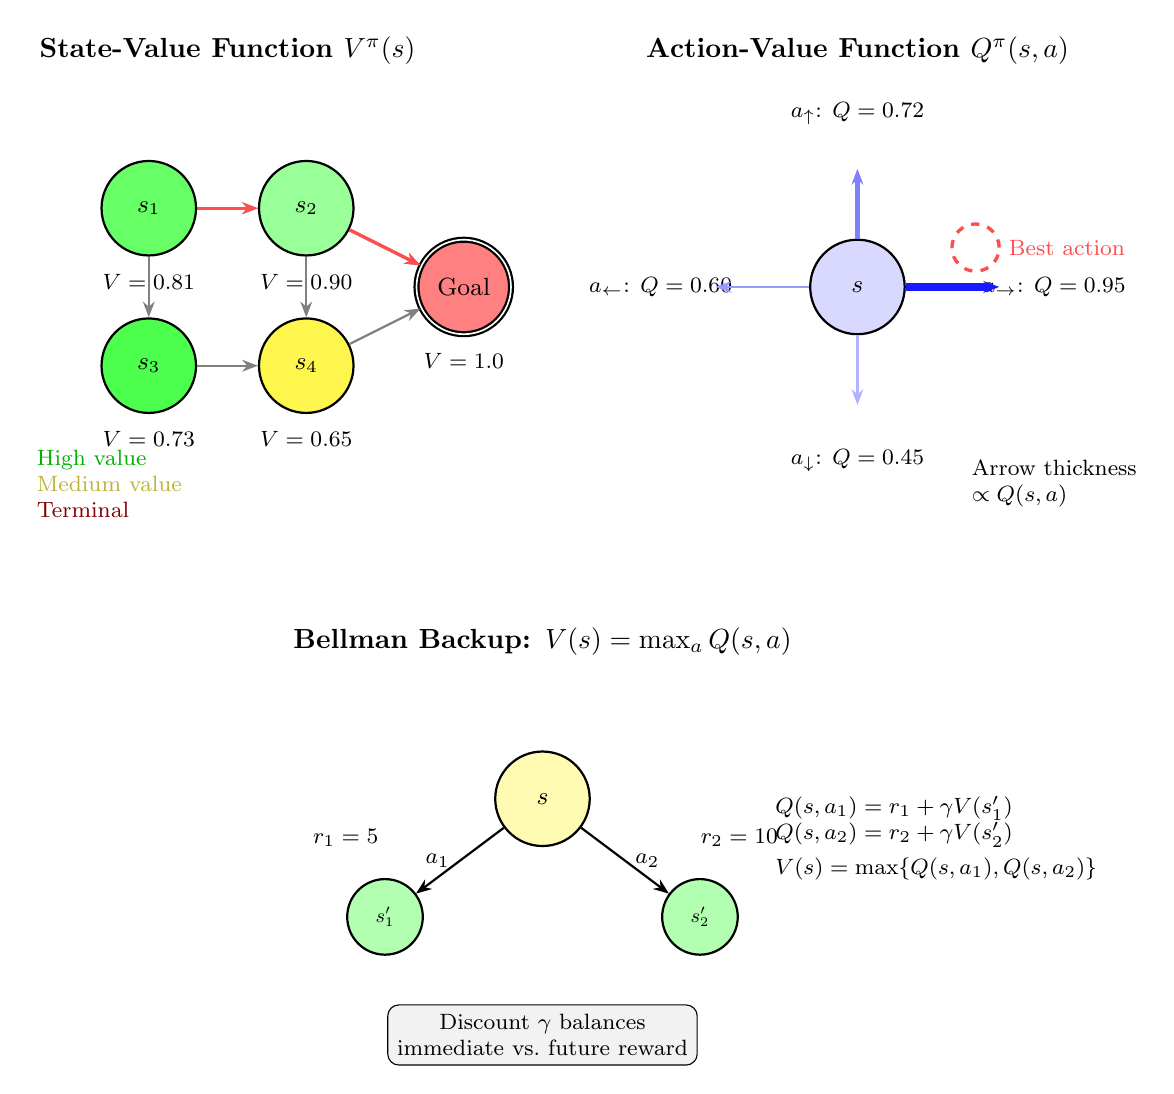
\begin{tikzpicture}[
    node distance=1.5cm,
    every node/.style={font=\small},
    state/.style={circle, draw, thick, minimum size=1.2cm, fill=blue!15},
    statevalue/.style={circle, draw, thick, minimum size=1.2cm},
    arrow/.style={-{Stealth[length=2mm]}, thick},
    label/.style={font=\footnotesize}
]

% ============ STATE-VALUE FUNCTION V(s) ============
\node[font=\bfseries] at (-5, 3) {State-Value Function $V^\pi(s)$};

% States with values (grid world example)
\node[statevalue, fill=green!60] (s1) at (-6, 1) {$s_1$};
\node[statevalue, fill=green!40] (s2) at (-4, 1) {$s_2$};
\node[statevalue, fill=green!70] (s3) at (-6, -1) {$s_3$};
\node[statevalue, fill=yellow!70] (s4) at (-4, -1) {$s_4$};
\node[statevalue, fill=red!50, double] (goal) at (-2, 0) {Goal};

% Value labels
\node[label, below=0.1cm of s1] {$V=0.81$};
\node[label, below=0.1cm of s2] {$V=0.90$};
\node[label, below=0.1cm of s3] {$V=0.73$};
\node[label, below=0.1cm of s4] {$V=0.65$};
\node[label, below=0.1cm of goal] {$V=1.0$};

% Transitions
\draw[arrow, gray] (s1) -- (s2);
\draw[arrow, gray] (s1) -- (s3);
\draw[arrow, gray] (s2) -- (s4);
\draw[arrow, gray] (s2) -- (goal);
\draw[arrow, gray] (s3) -- (s4);
\draw[arrow, gray] (s4) -- (goal);

% Optimal path highlight
\draw[arrow, red!70, very thick] (s1) -- (s2);
\draw[arrow, red!70, very thick] (s2) -- (goal);

% Color legend for V
\node[label, align=left] at (-6.5, -2.5) {
    \textcolor{green!70!black}{High value}\\
    \textcolor{yellow!70!black}{Medium value}\\
    \textcolor{red!50!black}{Terminal}
};

% ============ ACTION-VALUE FUNCTION Q(s,a) ============
\node[font=\bfseries] at (3, 3) {Action-Value Function $Q^\pi(s,a)$};

% Central state
\node[state] (center) at (3, 0) {$s$};

% Actions with Q-values
\node[label] at (3, 2.2) {$a_\uparrow$: $Q=0.72$};
\node[label] at (5.5, 0) {$a_\rightarrow$: $Q=0.95$};
\node[label] at (3, -2.2) {$a_\downarrow$: $Q=0.45$};
\node[label] at (0.5, 0) {$a_\leftarrow$: $Q=0.60$};

% Action arrows with thickness proportional to Q-value
\draw[arrow, blue!50, line width=1.5pt] (center) -- ++(0, 1.5) node[midway, right, font=\tiny] {};
\draw[arrow, blue!90, line width=3pt] (center) -- ++(1.8, 0) node[midway, above, font=\tiny] {};
\draw[arrow, blue!30, line width=0.8pt] (center) -- ++(0, -1.5) node[midway, right, font=\tiny] {};
\draw[arrow, blue!40, line width=1pt] (center) -- ++(-1.8, 0) node[midway, above, font=\tiny] {};

% Best action indicator
\draw[red!70, very thick, dashed] (4.5, 0.5) circle (0.3);
\node[label, red!70, right] at (4.8, 0.5) {Best action};

% Arrow thickness legend
\node[label, align=left] at (5.5, -2.5) {
    Arrow thickness\\
    $\propto Q(s,a)$
};

% ============ BELLMAN BACKUP ILLUSTRATION ============
\node[font=\bfseries] at (-1, -4.5) {Bellman Backup: $V(s) = \max_a Q(s,a)$};

% States showing backup
\node[state, fill=yellow!30] (bs) at (-1, -6.5) {$s$};
\node[state, fill=green!30, scale=0.8] (bs1) at (-3, -8) {$s'_1$};
\node[state, fill=green!30, scale=0.8] (bs2) at (1, -8) {$s'_2$};

% Backup arrows
\draw[arrow] (bs) -- node[left, label] {$a_1$} (bs1);
\draw[arrow] (bs) -- node[right, label] {$a_2$} (bs2);

% Reward and transition
\node[label] at (-3.5, -7) {$r_1=5$};
\node[label] at (1.5, -7) {$r_2=10$};

% Value computation
\node[label, align=left] at (4, -7) {
    $Q(s,a_1) = r_1 + \gamma V(s'_1)$\\
    $Q(s,a_2) = r_2 + \gamma V(s'_2)$\\[3pt]
    $V(s) = \max\{Q(s,a_1), Q(s,a_2)\}$
};

% Discount factor annotation
\node[draw, rounded corners, fill=gray!10, label, align=center] at (-1, -9.5) {
    Discount $\gamma$ balances\\
    immediate vs.\ future reward
};

\end{tikzpicture}
\end{document}
